
\documentclass[11pt]{article}
\usepackage{amsmath,amssymb}
\usepackage{graphicx}
\usepackage{natbib}
\usepackage[parfill]{parskip}
\usepackage[margin=1in]{geometry}
\usepackage{pdflscape}
\title{Supplementary information for ``CLM5-PPE"}
\author{D. Kennedy}
\renewcommand{\thefigure}{S\arabic{figure}}
\begin{document}
\maketitle


\begin{figure}[h]
\centering
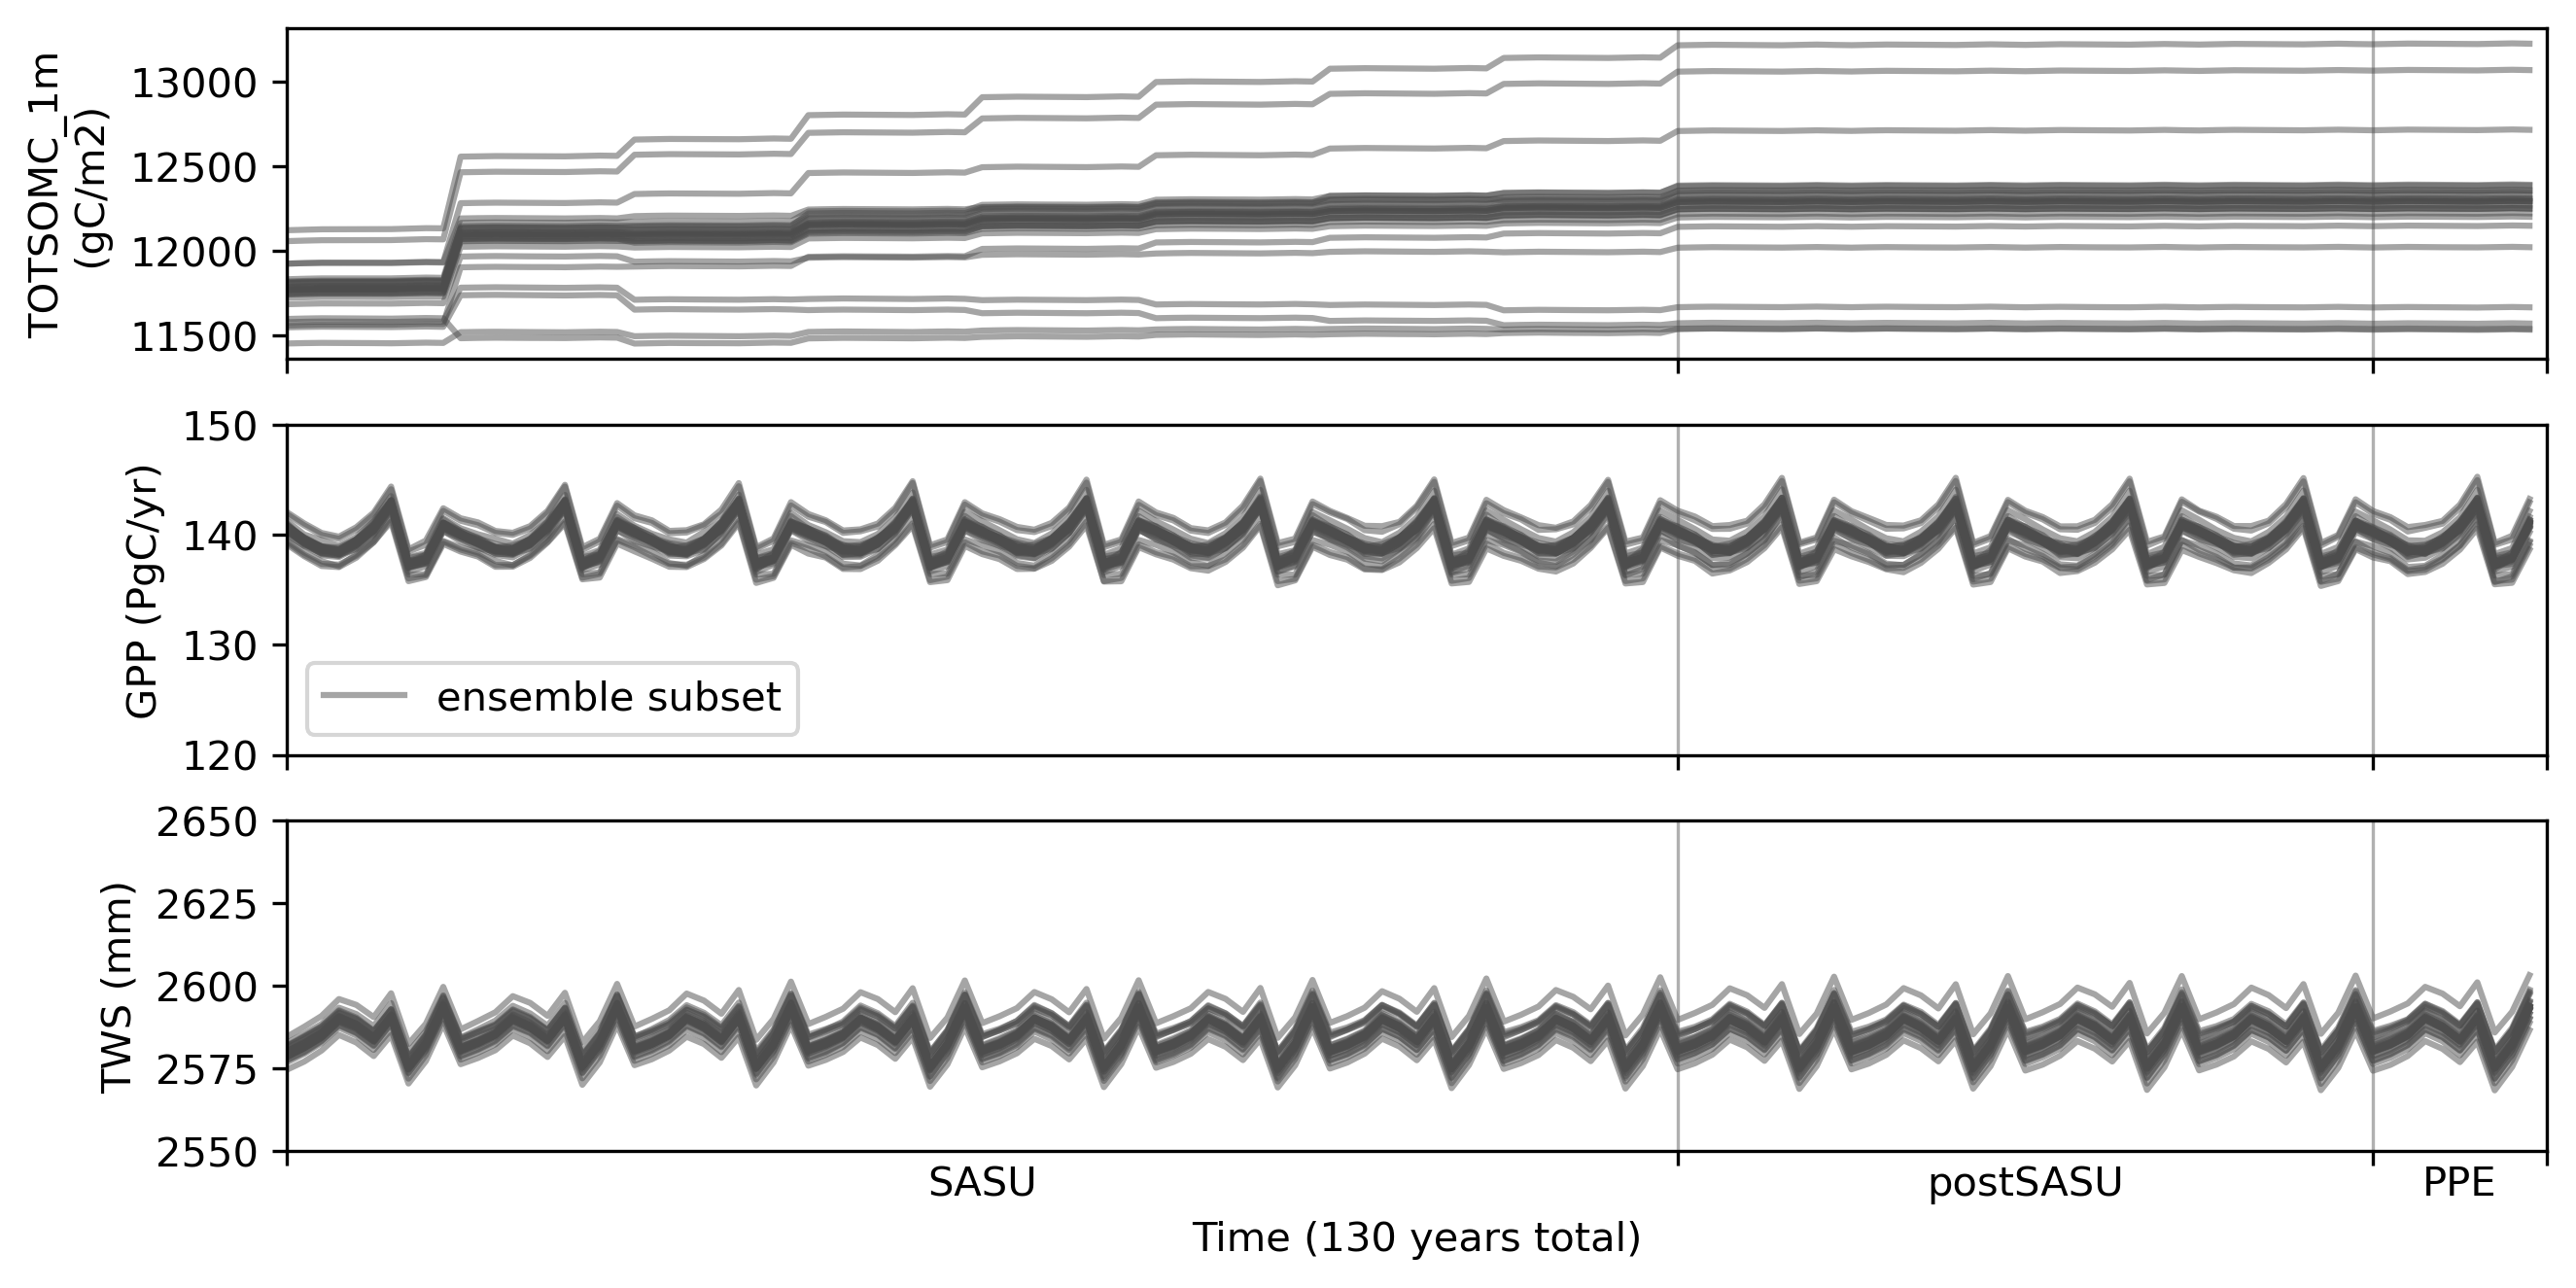
\includegraphics[width=40pc]{../figs/supp/spinup.png}
\caption{Independent spinup was performed for each simulation of the ensemble. Whereas gross primary production (GPP) and total water storage (TWS) equilibrated quickly, total carbon soil organic matter in the top meter of the soil column (TOTSOMC\_1m) required longer spinup and did not always reach equilibrium.}
\label{supp:spinup}
\end{figure}


\begin{landscape}
\begin{figure}[h]
\centering
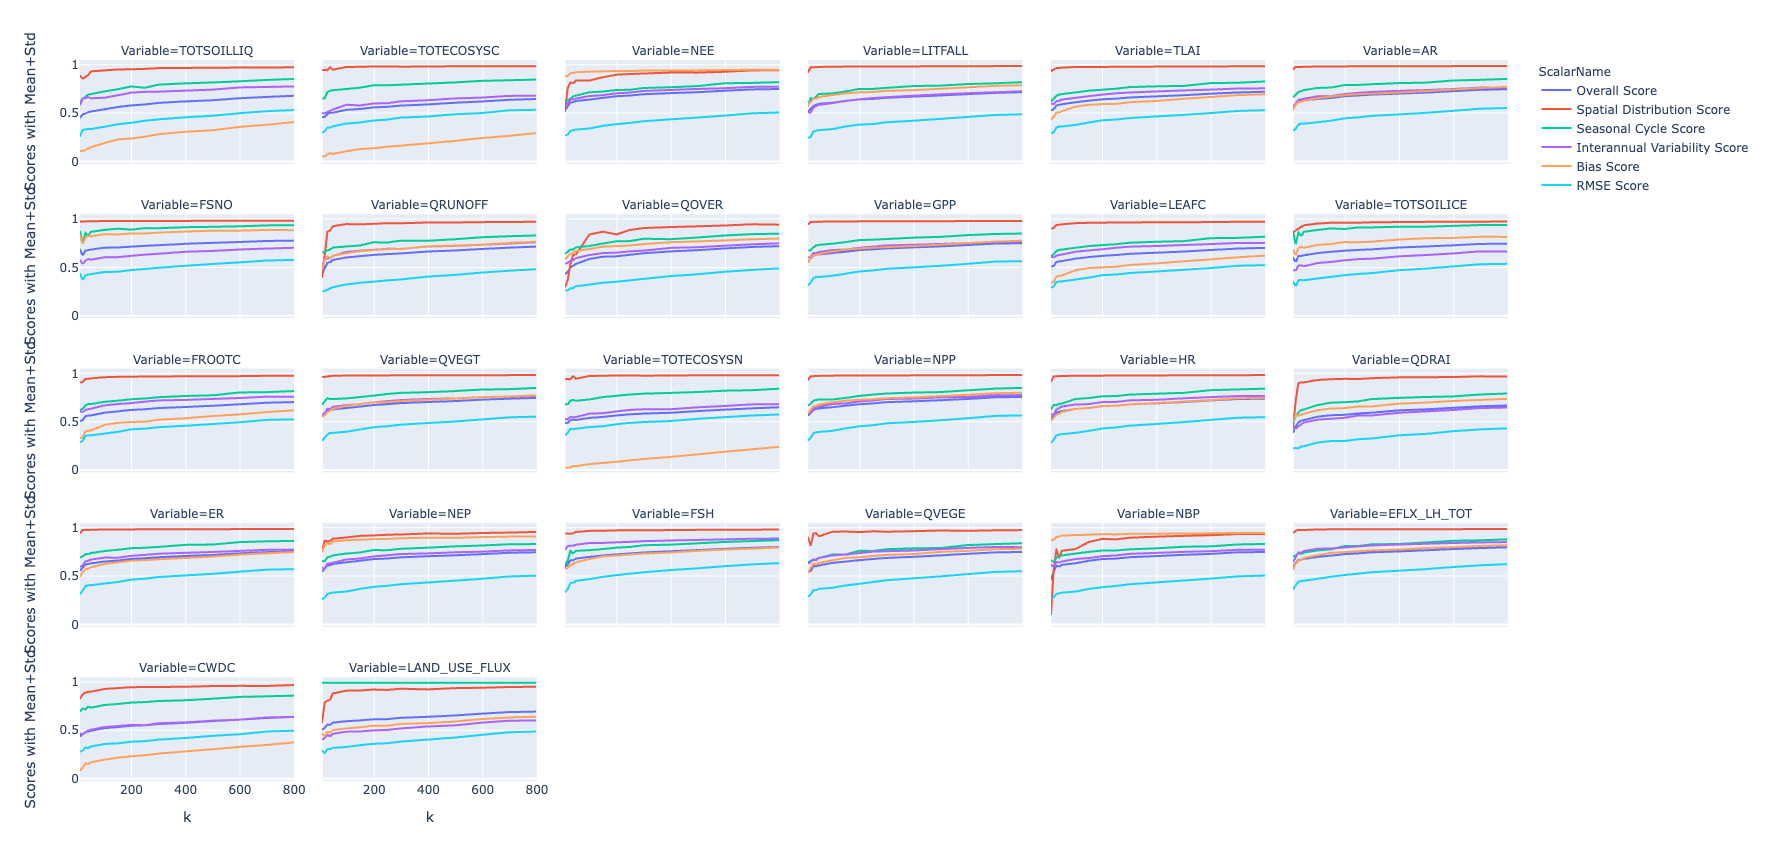
\includegraphics[width=60pc]{../figs/supp/ilamb_lines.png}
\caption{The convergence of several scoring metrics with increasing sparsegrid resolution across a variety of CLM variables. All scores tend towards 1 as the number of sparsegrid clusters (k) approaches the 5666 gridcells for the native resolution of our 2-degree simulations. }
\label{supp:ilamb}
\end{figure}
\end{landscape}



\begin{landscape}
\begin{figure}[h]
\centering
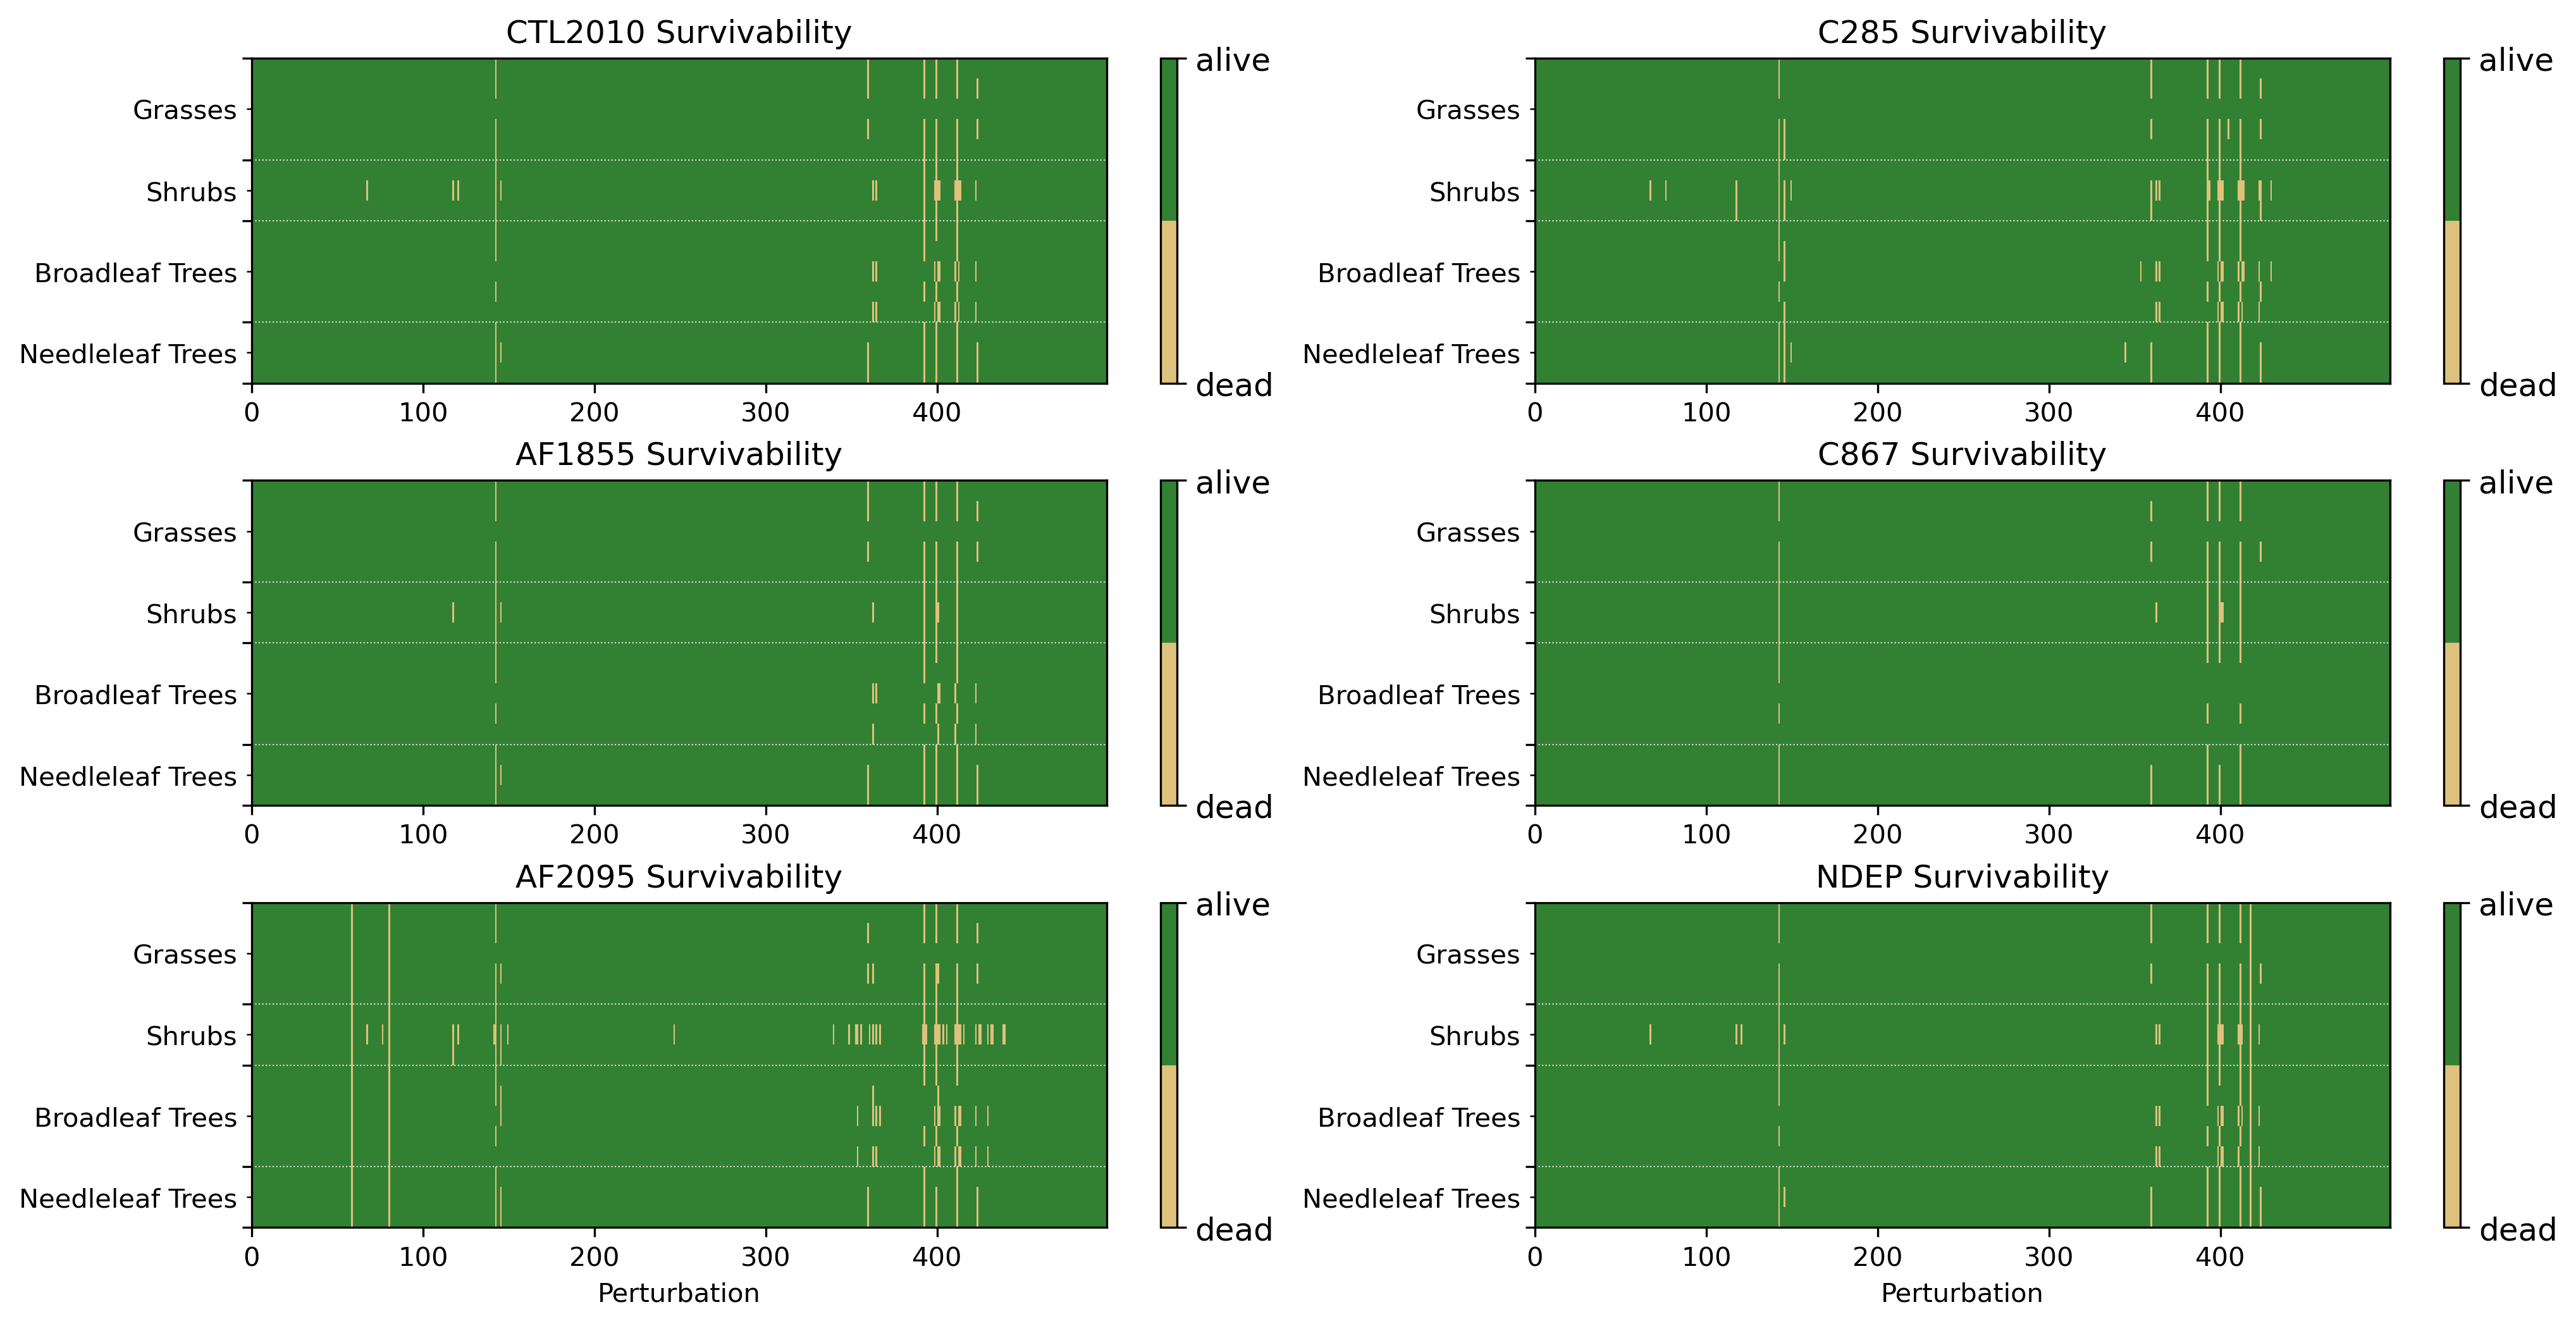
\includegraphics[width=50pc]{../figs/supp/survivability.png}
\caption{PFT survivability across the six ensembles. The sixteen natural vegetation PFTs are on the vertical axis, and the perturbation number sets the horizontal axis. A PFT is classified as dead in a given gridcell if it does not achieve an LAI of at least 0.1 m2/m2 at any point during the simulation. A PFT is classified as dead for a given perturbation if more than 50\% of the area that was alive with the default parameters is dead in the perturbed simulation.}
\label{supp:surv}
\end{figure}
\end{landscape}

\begin{figure}[h]
\centering
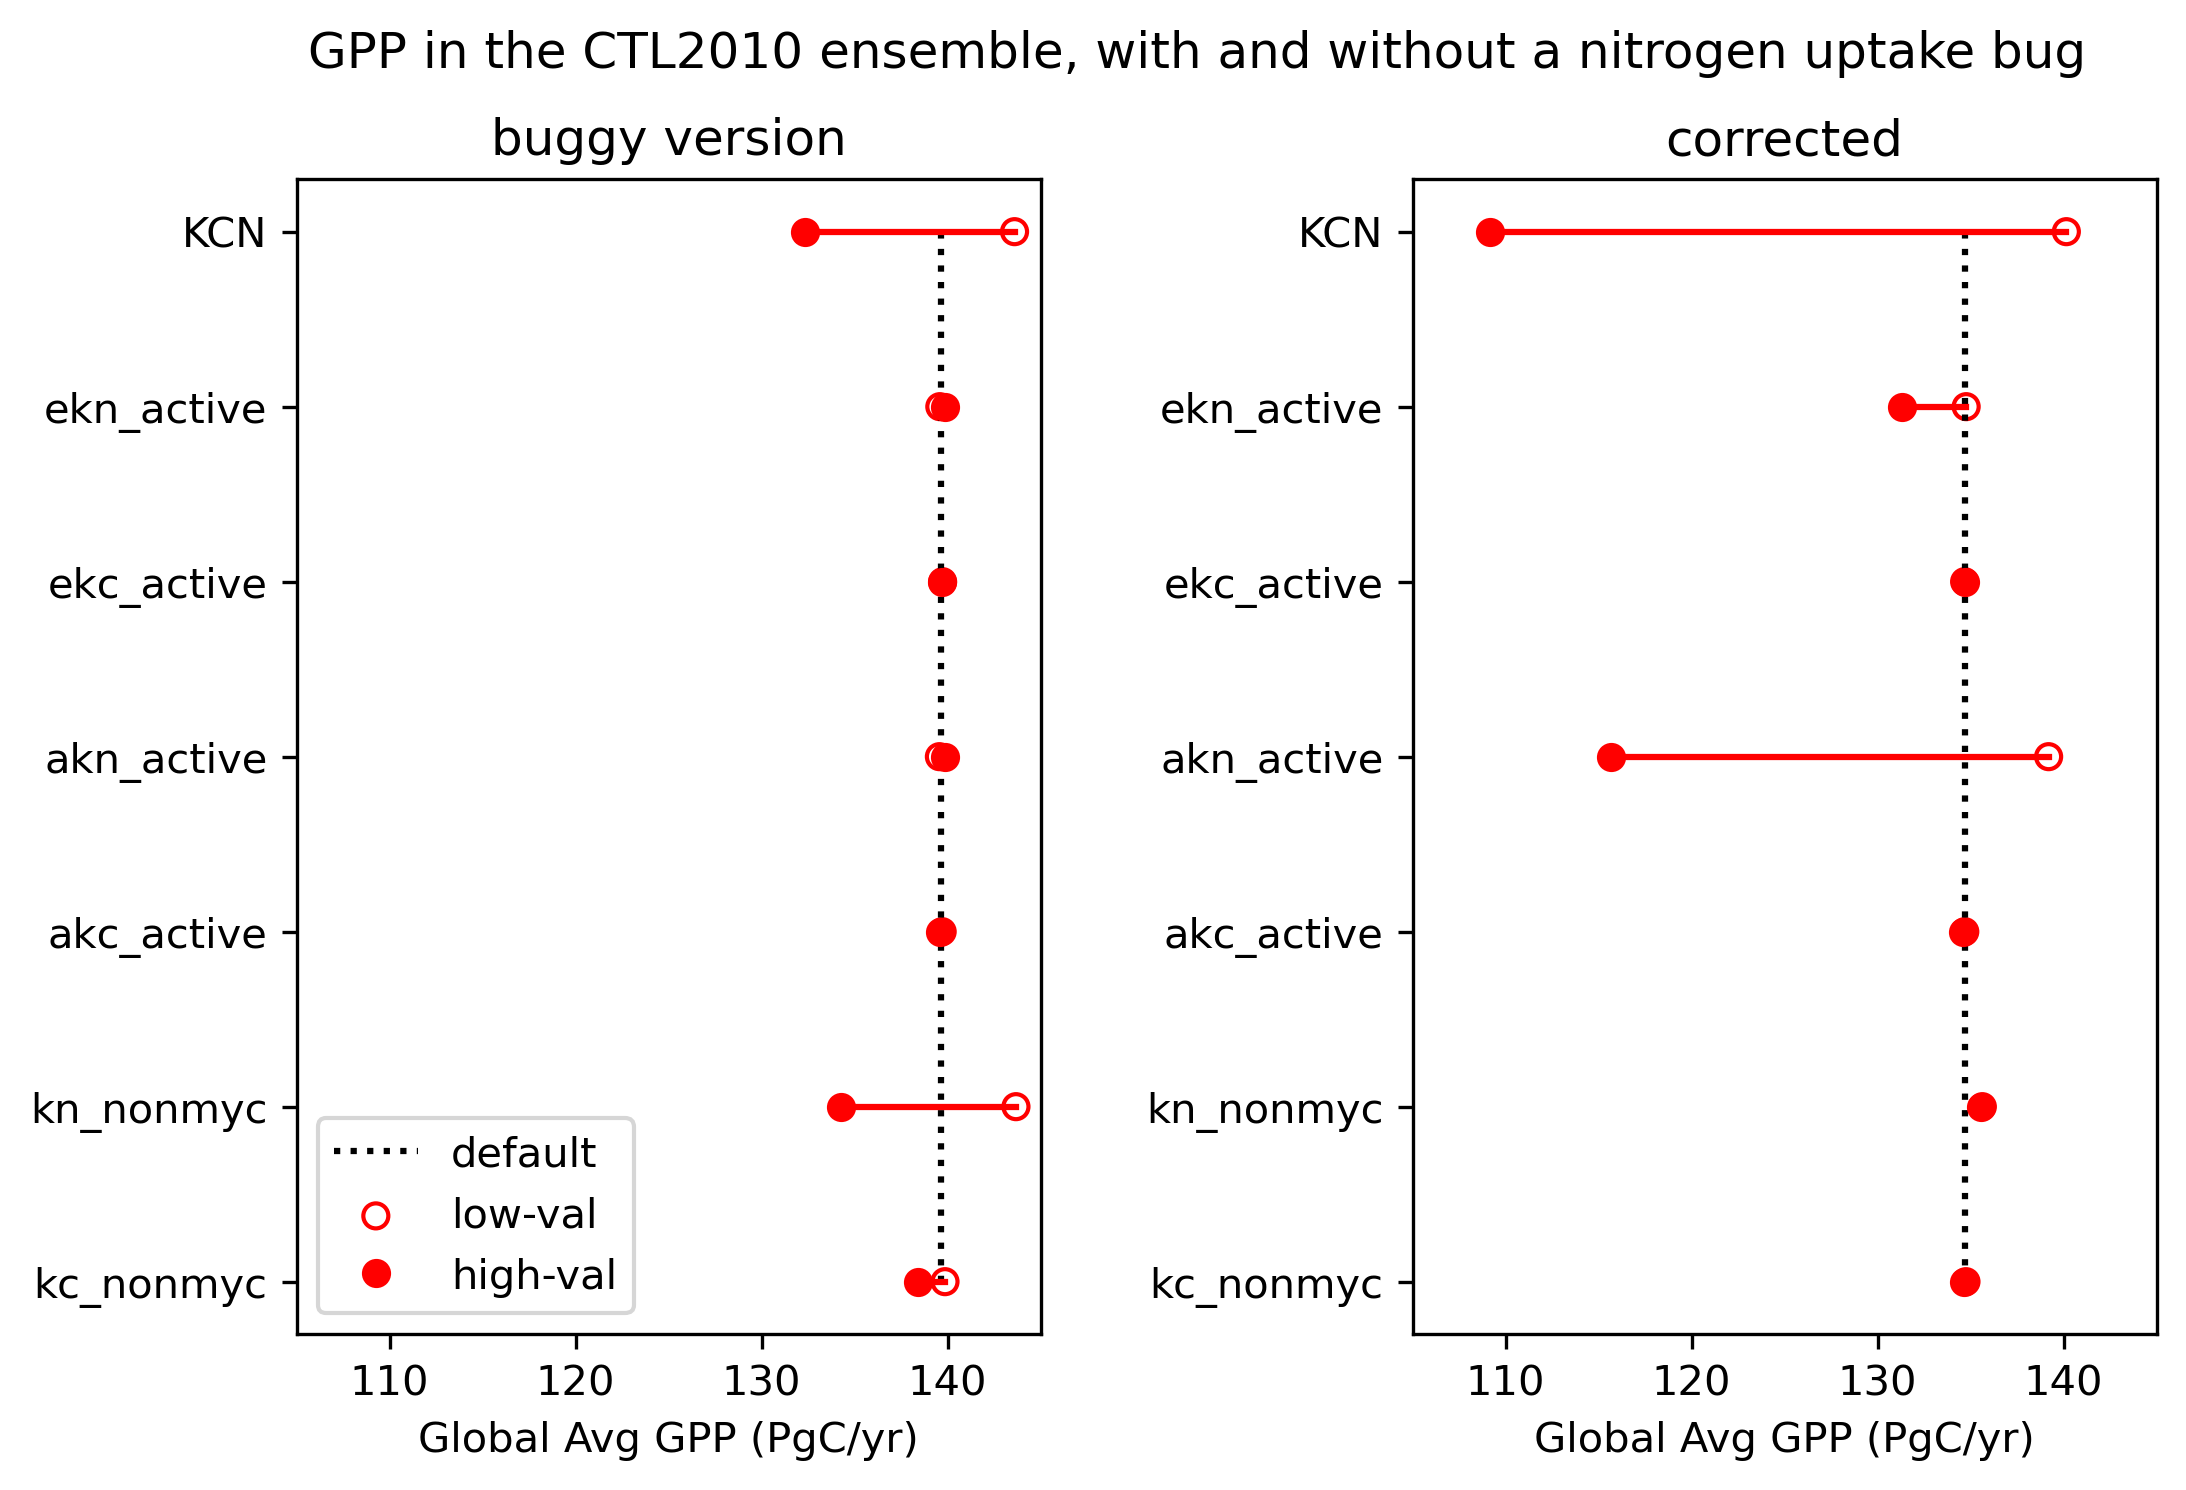
\includegraphics[width=\textwidth]{../figs/supp/funbug.png}
\caption{Parameter rankings for nitrogen uptake parameters subject to a recently uncovered CLM bug. The values for \textit{kn\_nonmyc} and \textit{kc\_nonmyc} had been accidentally transposed.}
\label{supp:funbug}
\end{figure}

\begin{figure}[h]
\centering
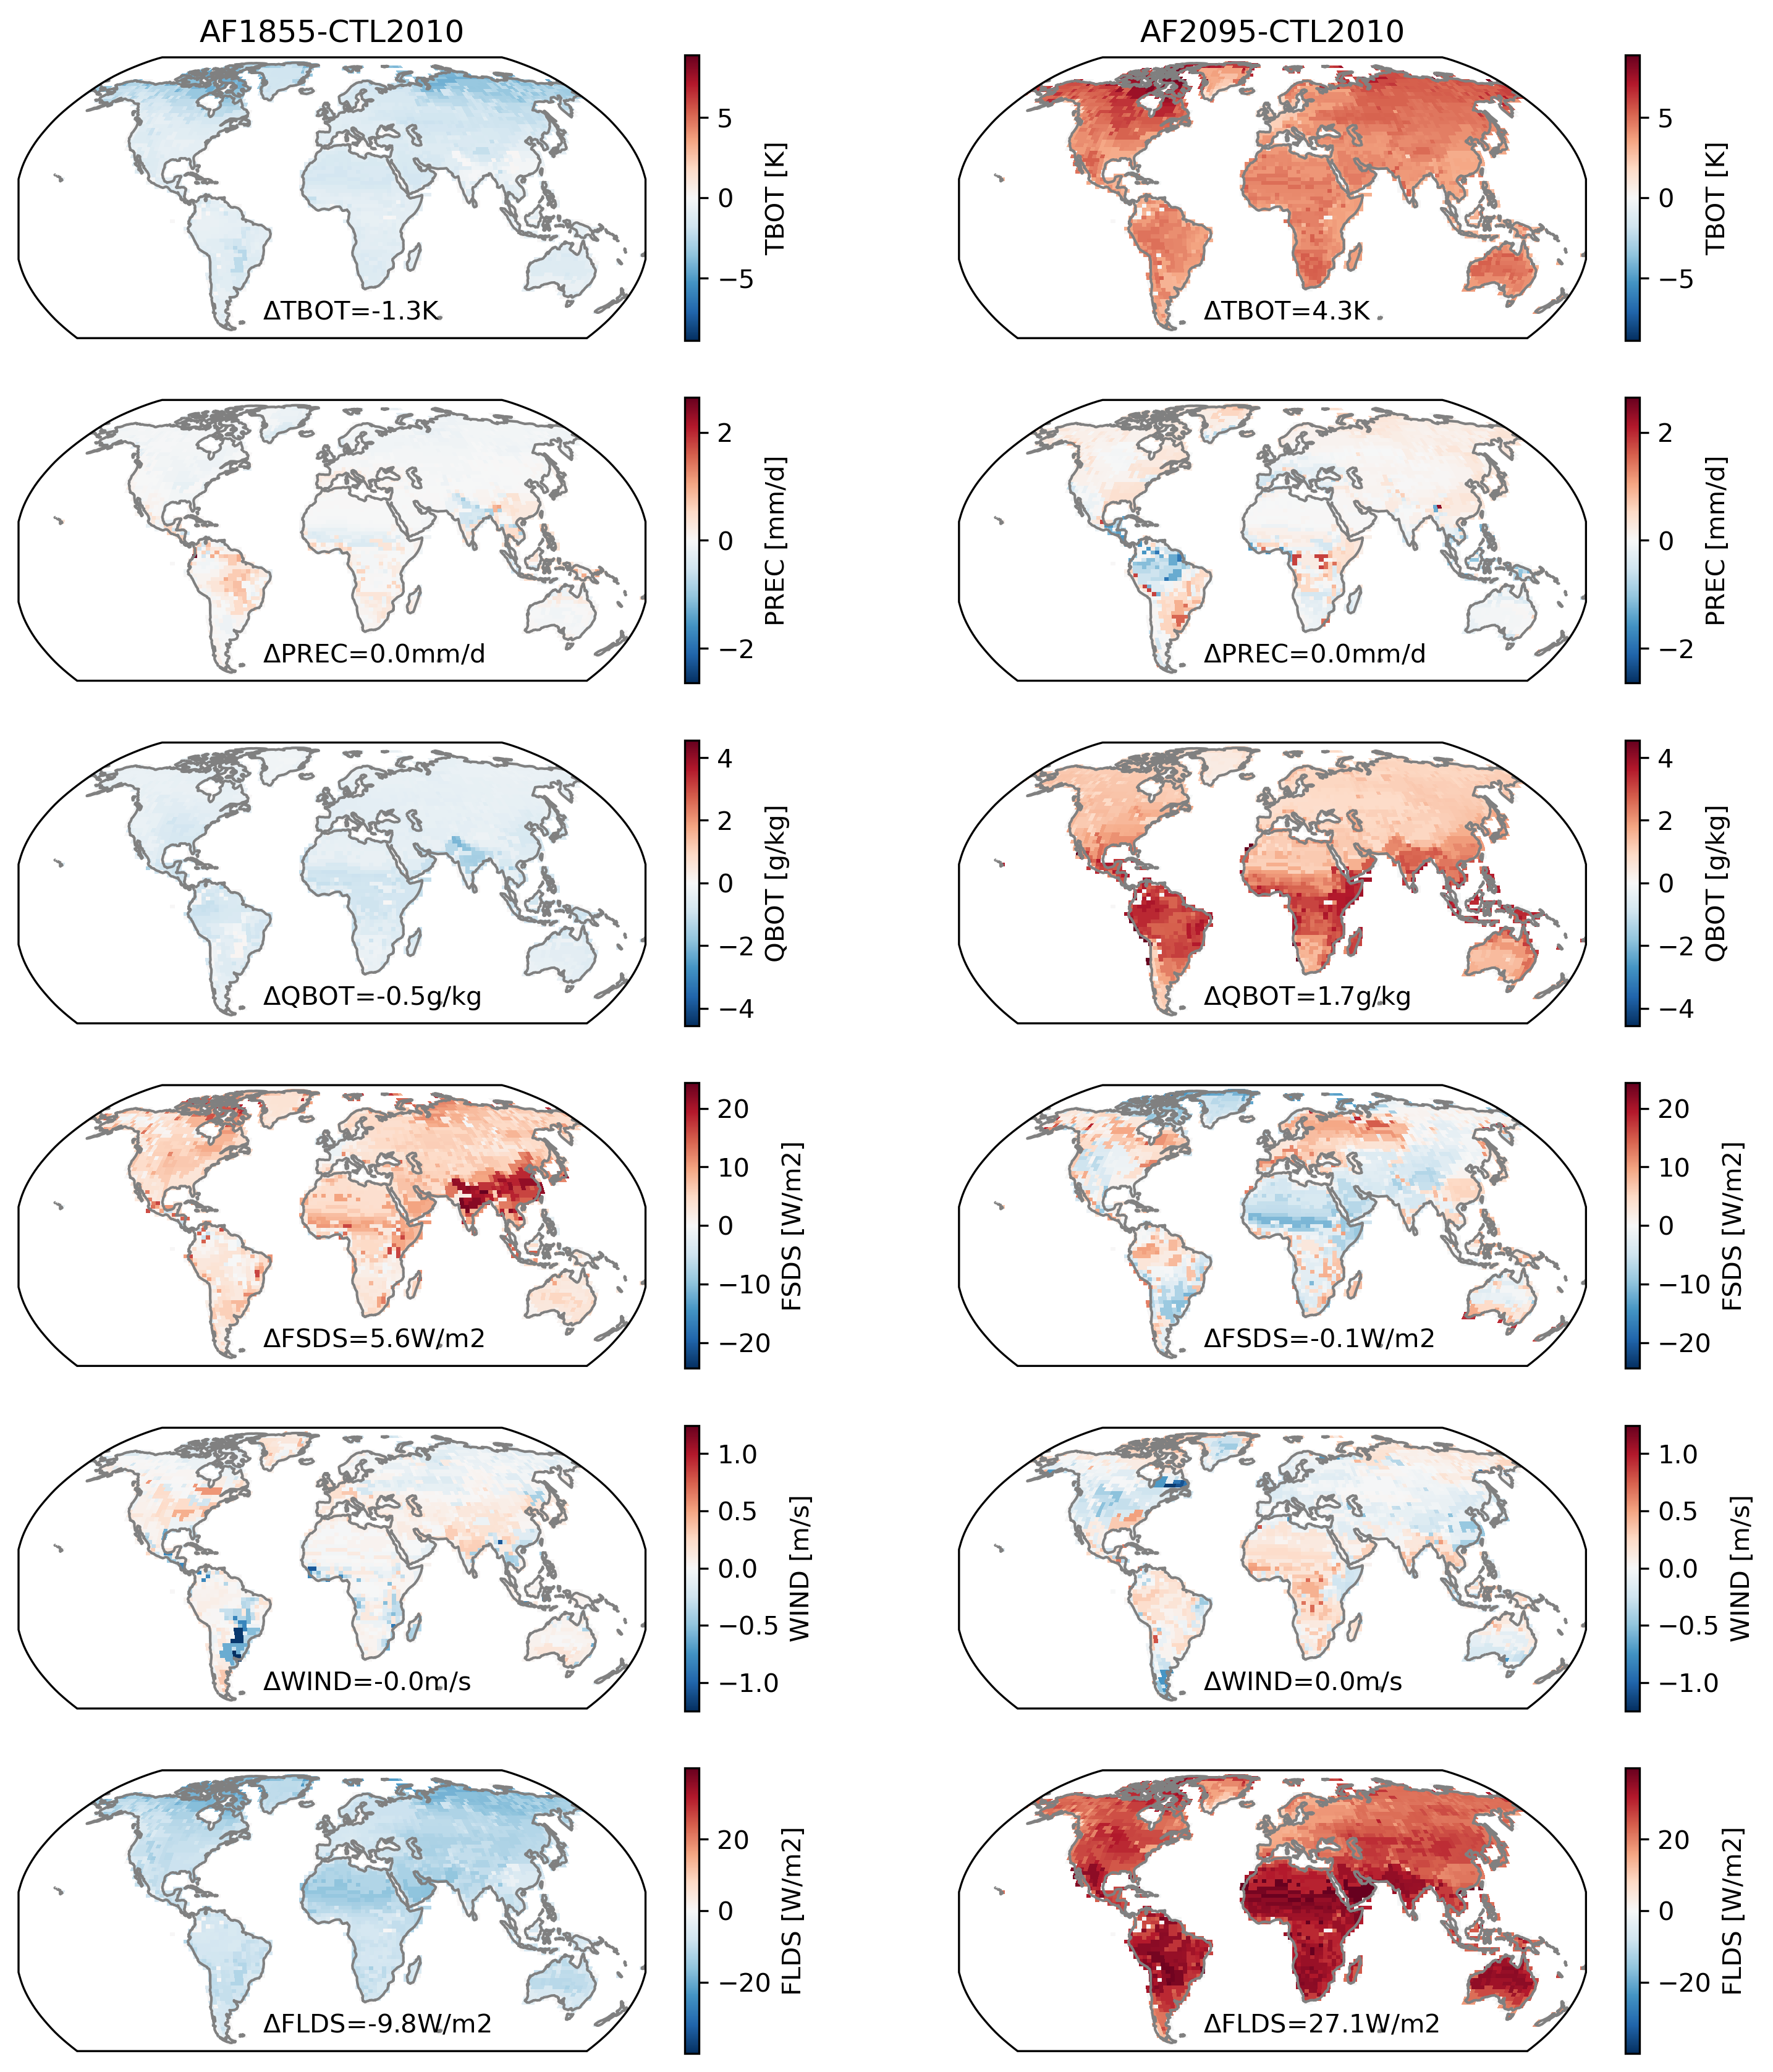
\includegraphics[width=\textwidth]{../figs/supp/anomalies.png}
\caption{Maps of average forcing anomalies in the pre-industrial (left column) and future climate forcing (right column) simulations. Global averages over land, Antarctica excluded, are written in text on each subplot.}
\label{supp:anomalies}
\end{figure}

\begin{figure}[h]
\centering
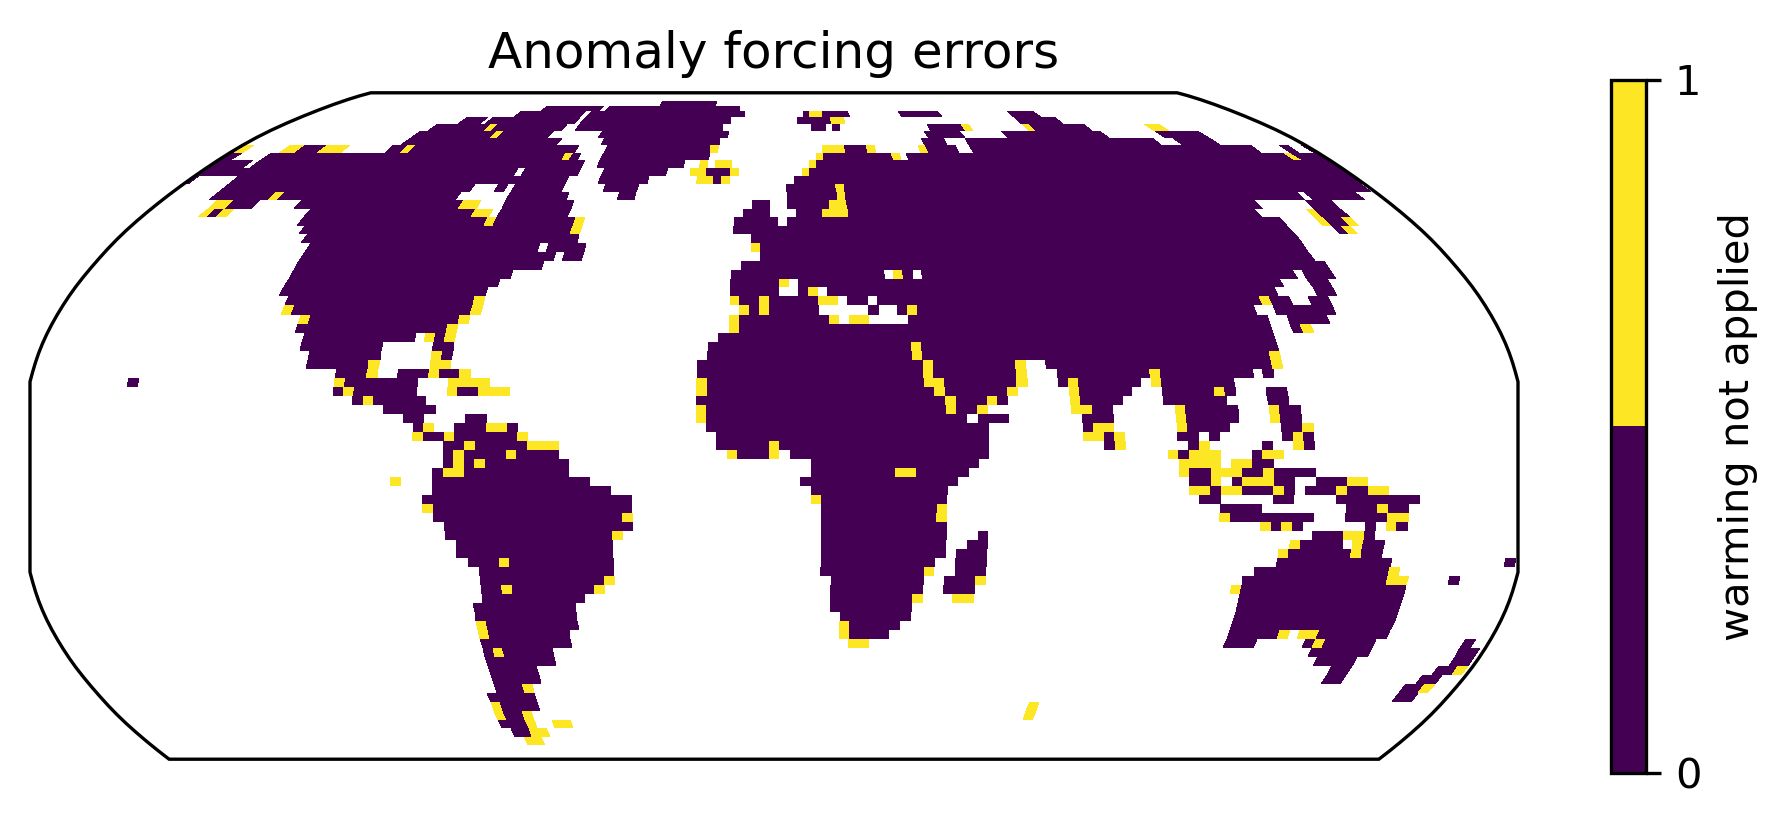
\includegraphics[width=\textwidth]{../figs/supp/anomaly_errors.png}
\caption{Due to a software error, certain gridcells (yellow) were not appropriately processed to receive climate anomalies for the AF1855 and AF2095 simulations. Instead those gridcells experience the control climate. In total these errant gridcells total less than 3\% of global land area.  }
\label{supp:abug}
\end{figure}

\begin{figure}[h]
\centering
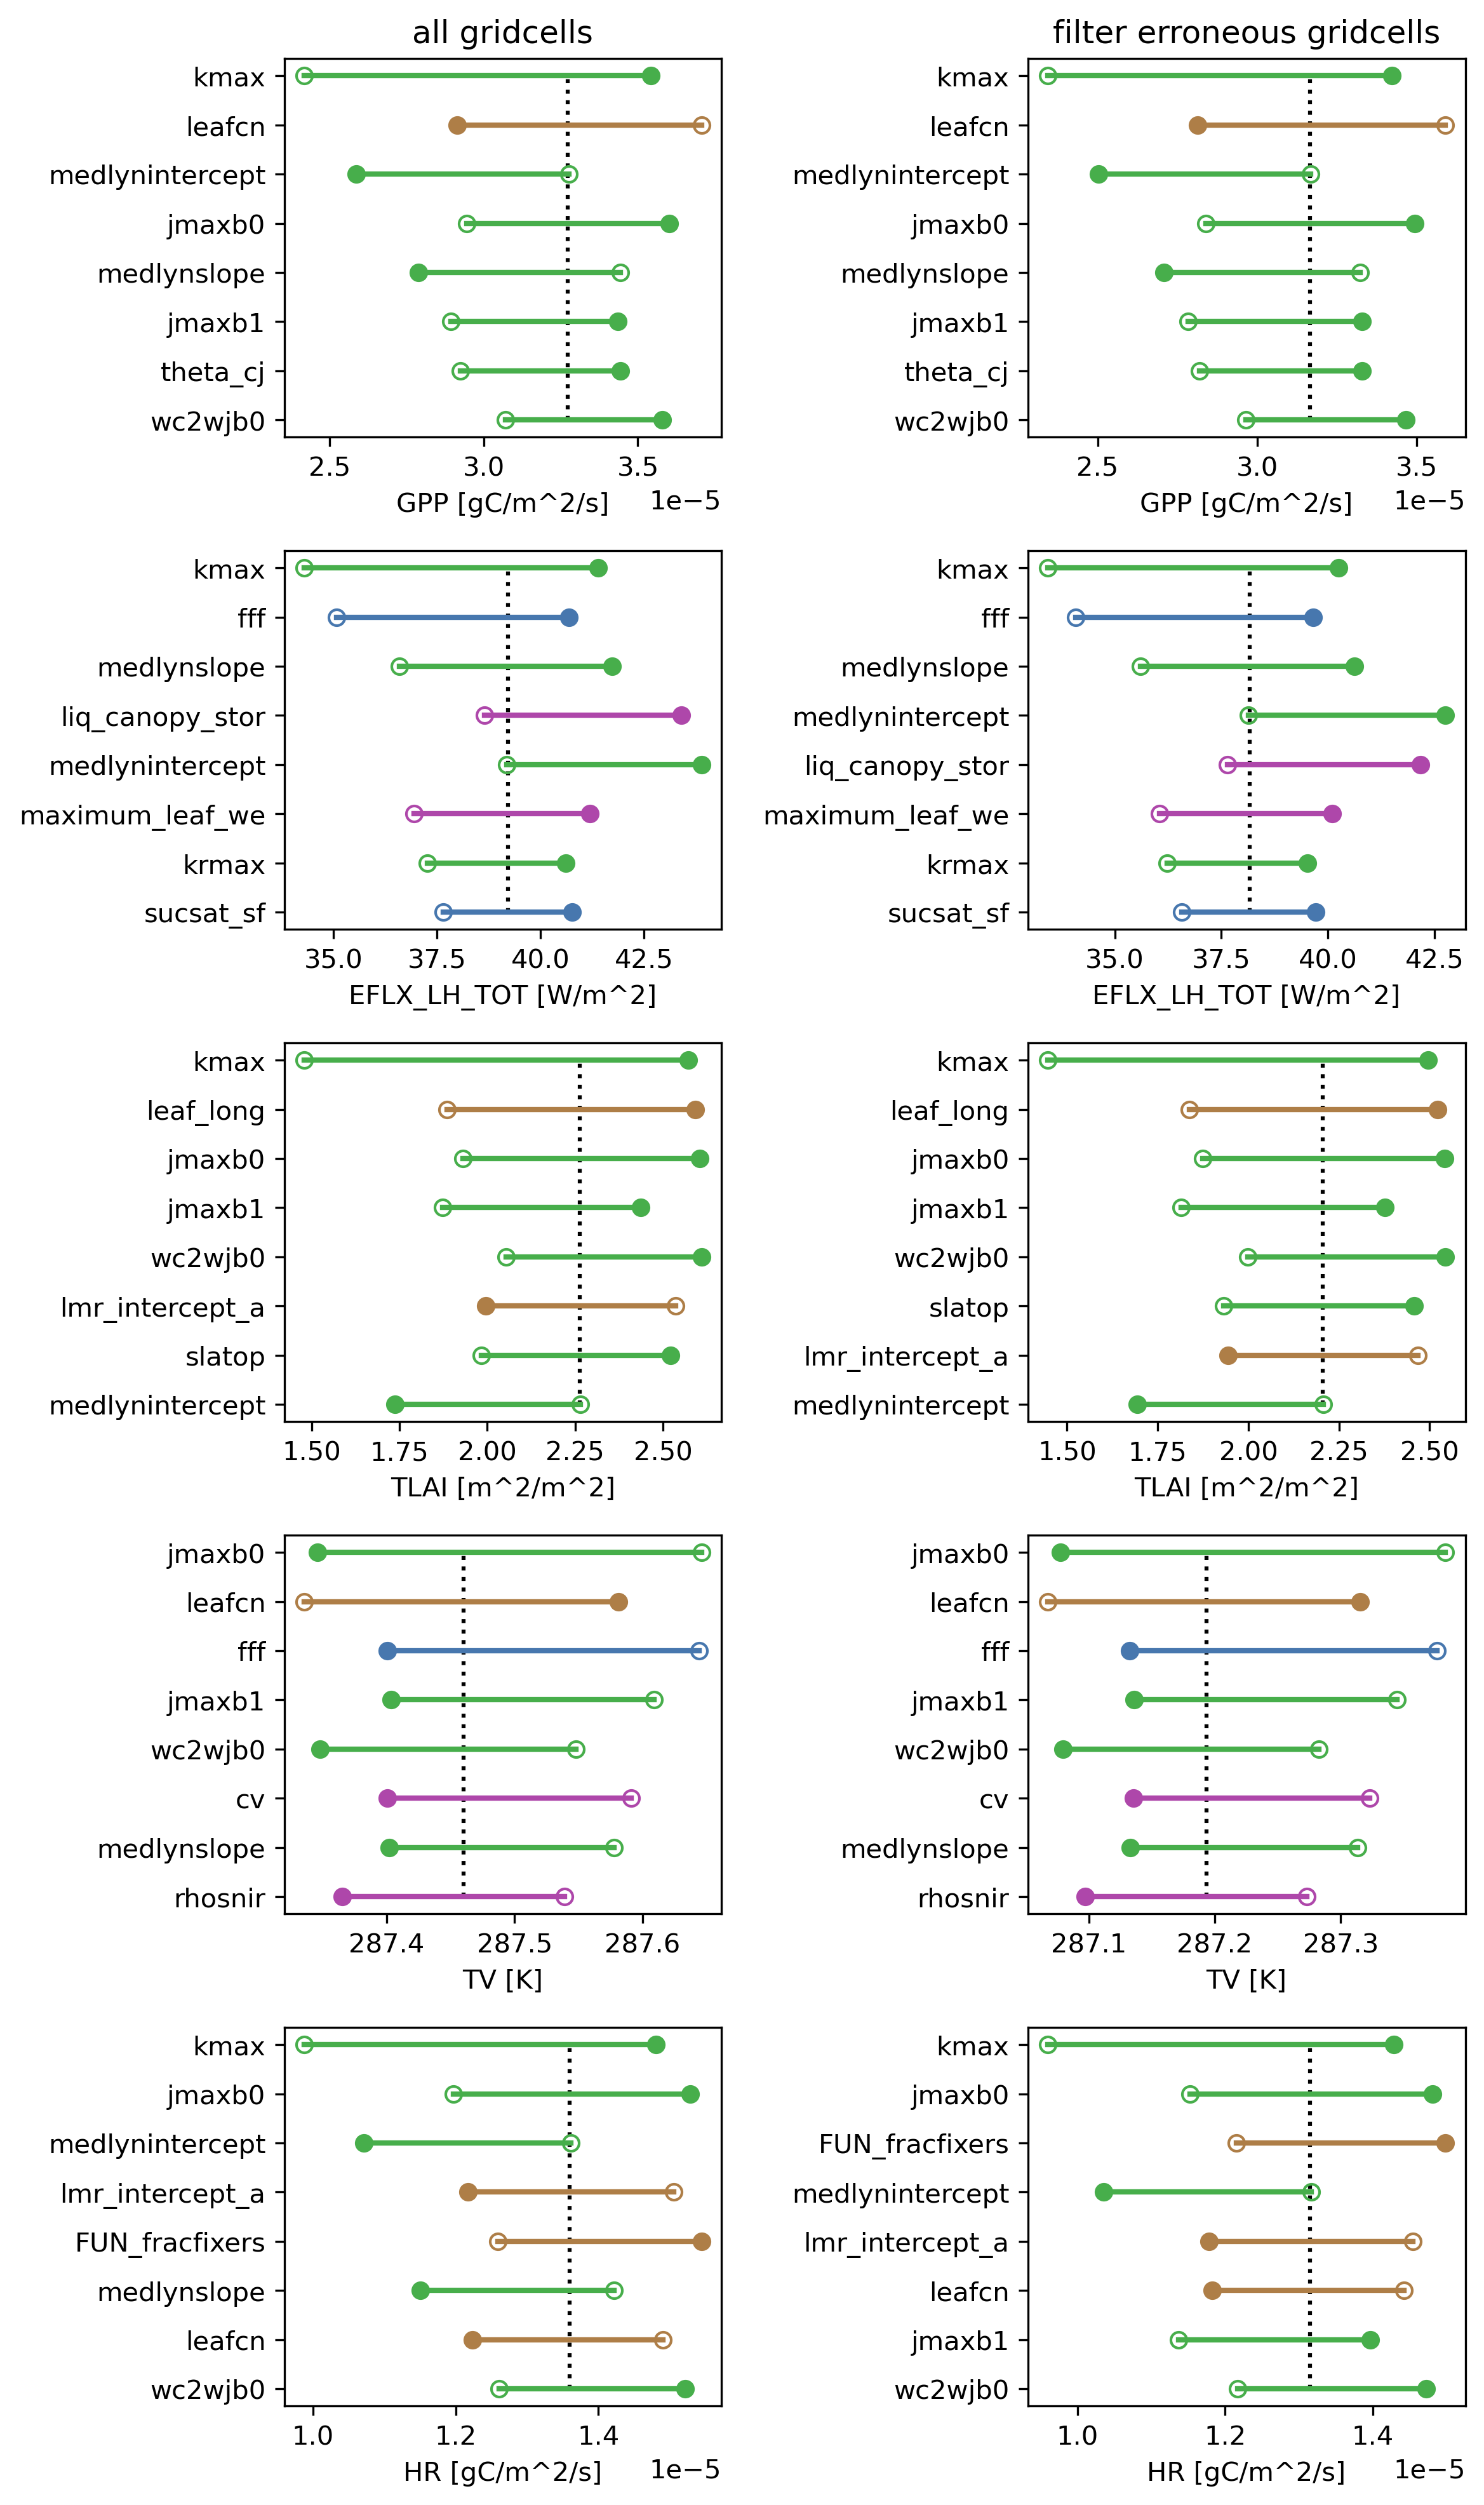
\includegraphics[width=30pc]{../figs/supp/AF2095_rankings.png}
\caption{Comparing parameter rankings with and without the errant gridcells from Supp Figure S6 across a selection of output variables.}
\label{supp:abug}
\end{figure}


\begin{figure}[h]
\centering
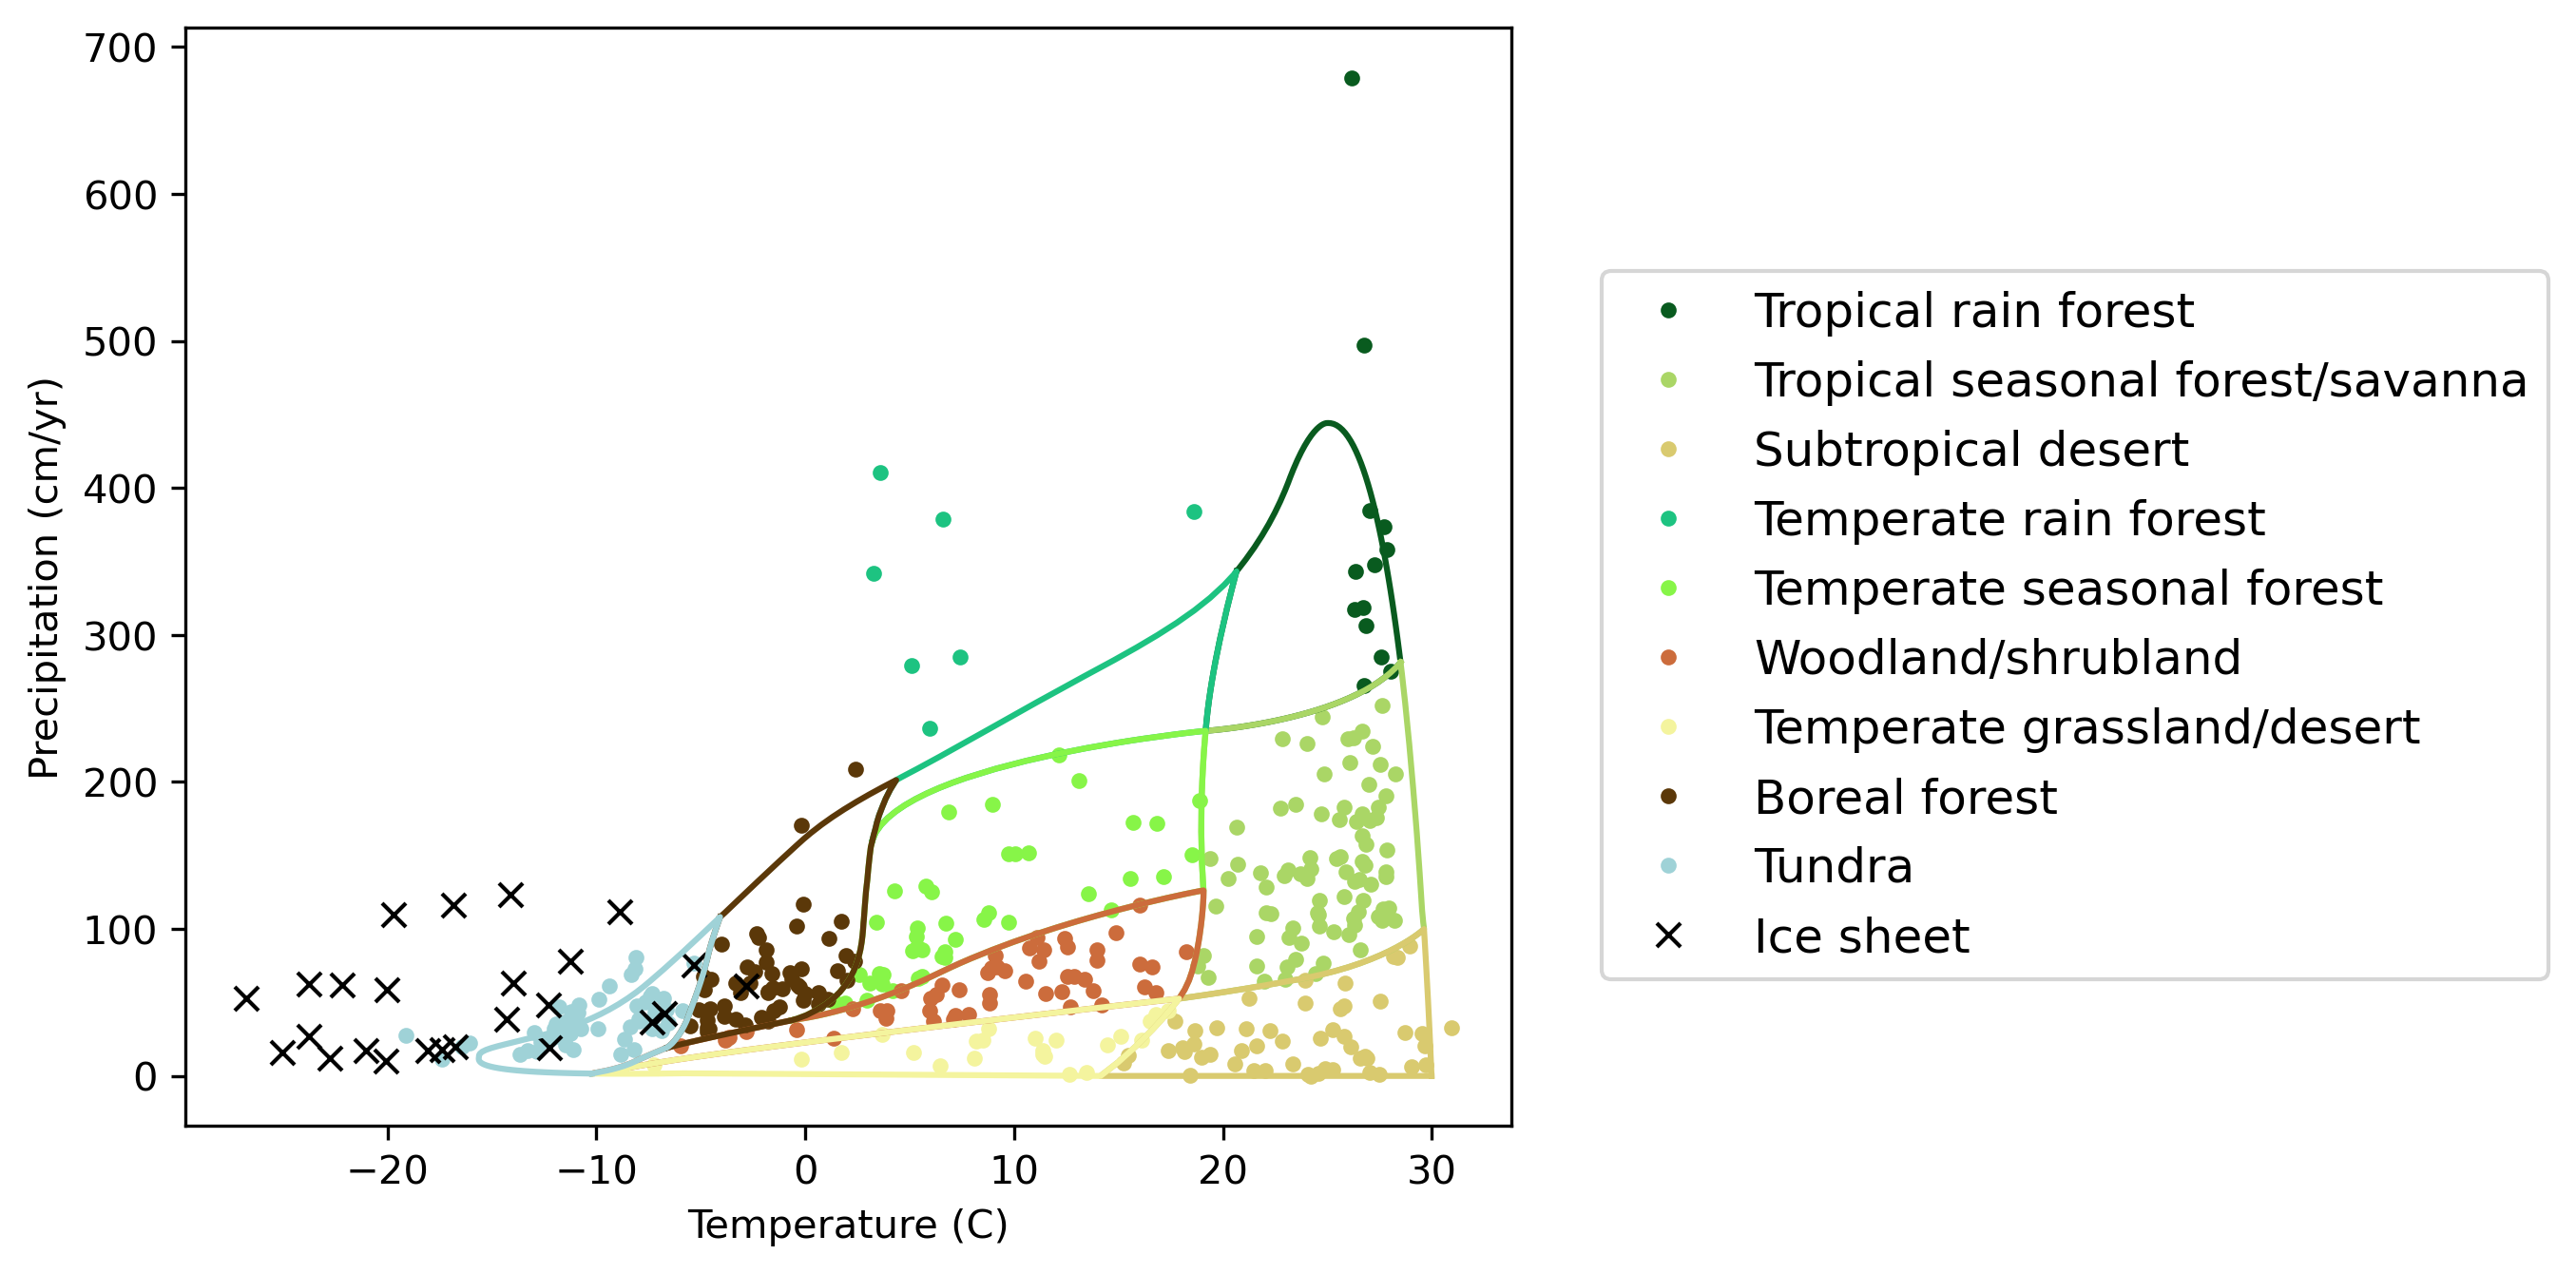
\includegraphics[width=40pc]{../figs/supp/biome_tp.png}
\caption{Each of the 400 sparse gridcells plotted according to their Whittaker biomes.}
\label{supp:whit1}
\end{figure}

\begin{figure}[h]
\centering
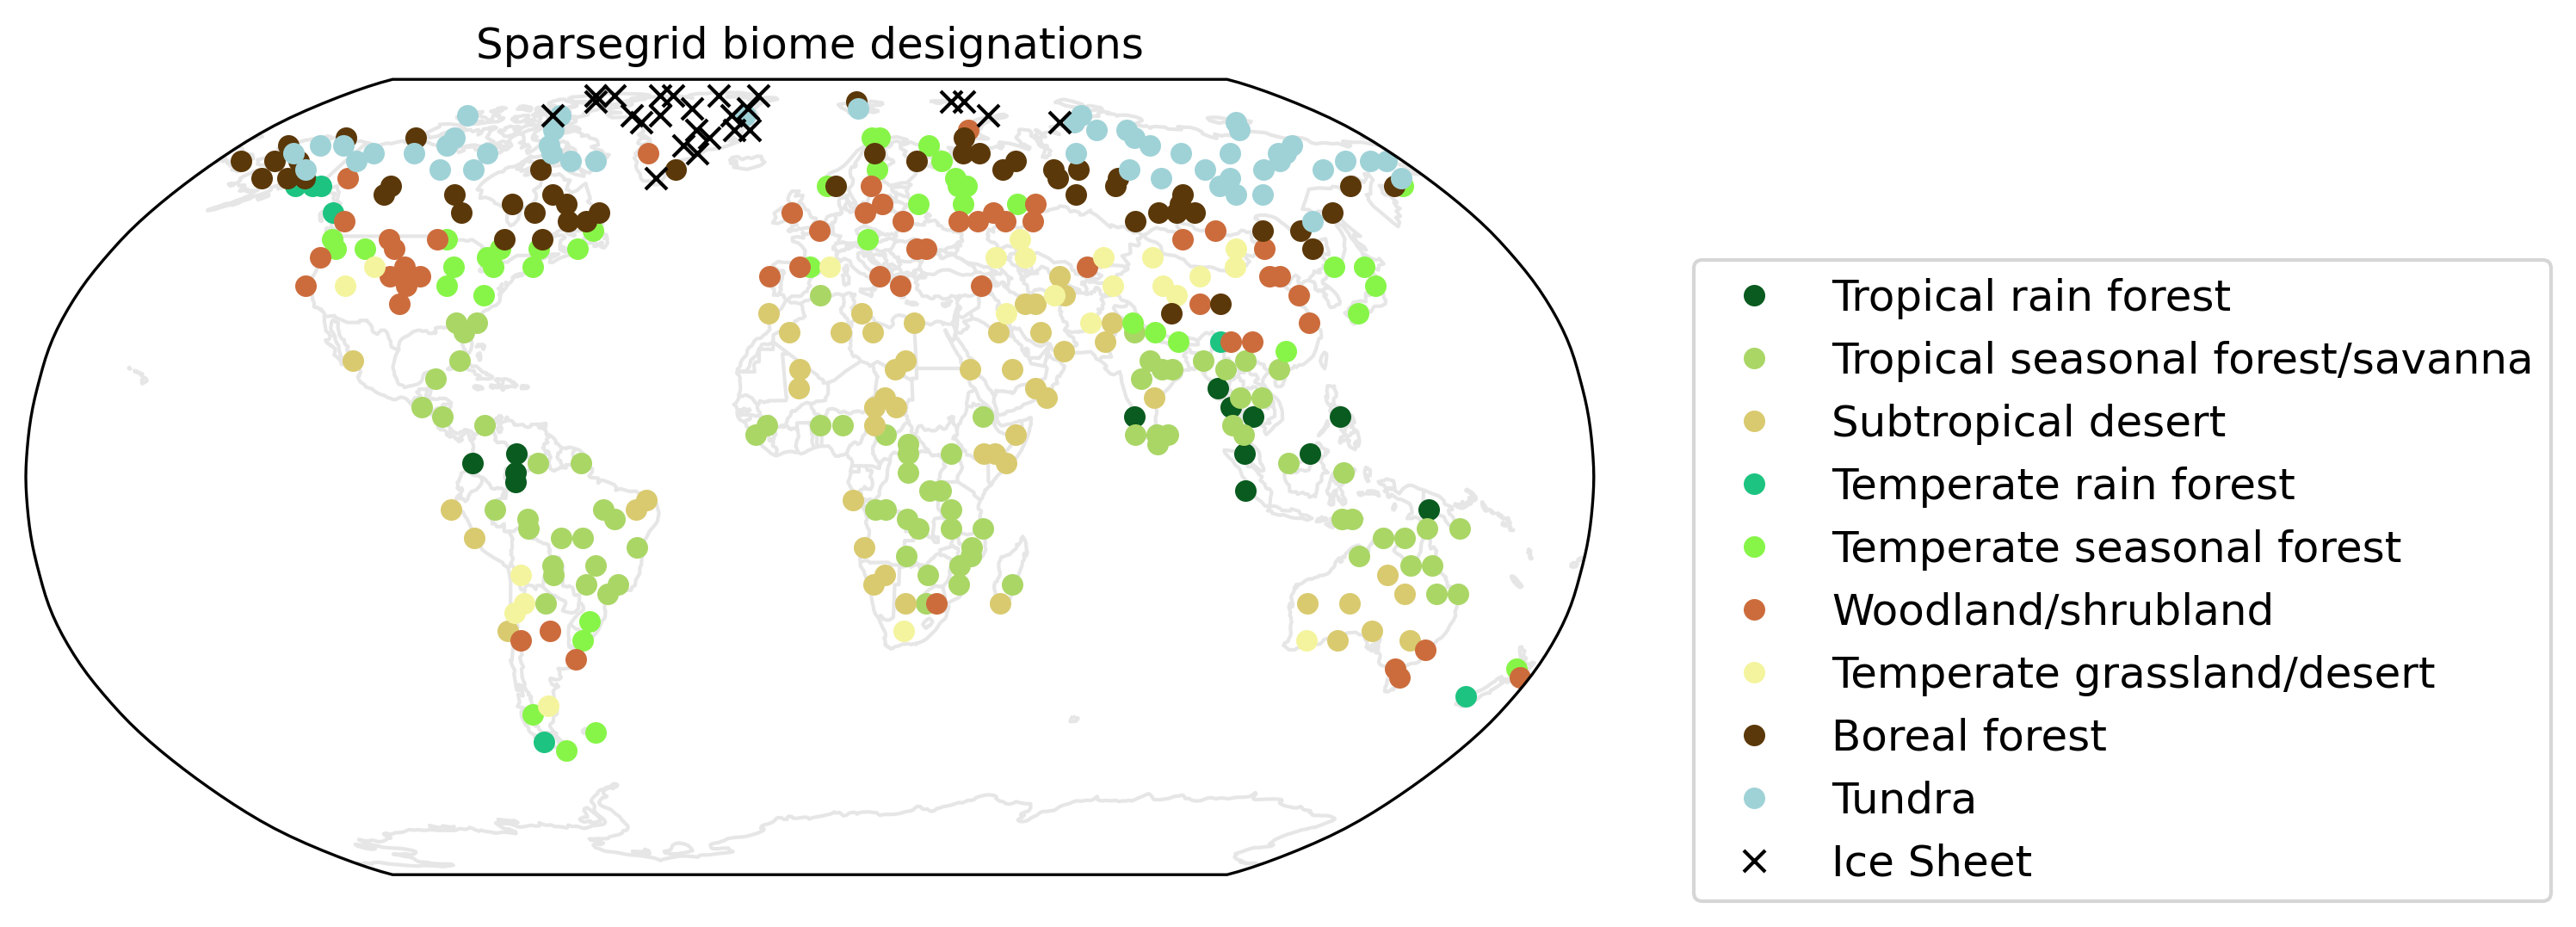
\includegraphics[width=40pc]{../figs/supp/biome_latlon.png}
\caption{Cartesian plot of the 400 sparse gridcells labeled by their Whittaker biomes.}
\label{supp:whit2}
\end{figure}


\begin{figure}[h]
\centering
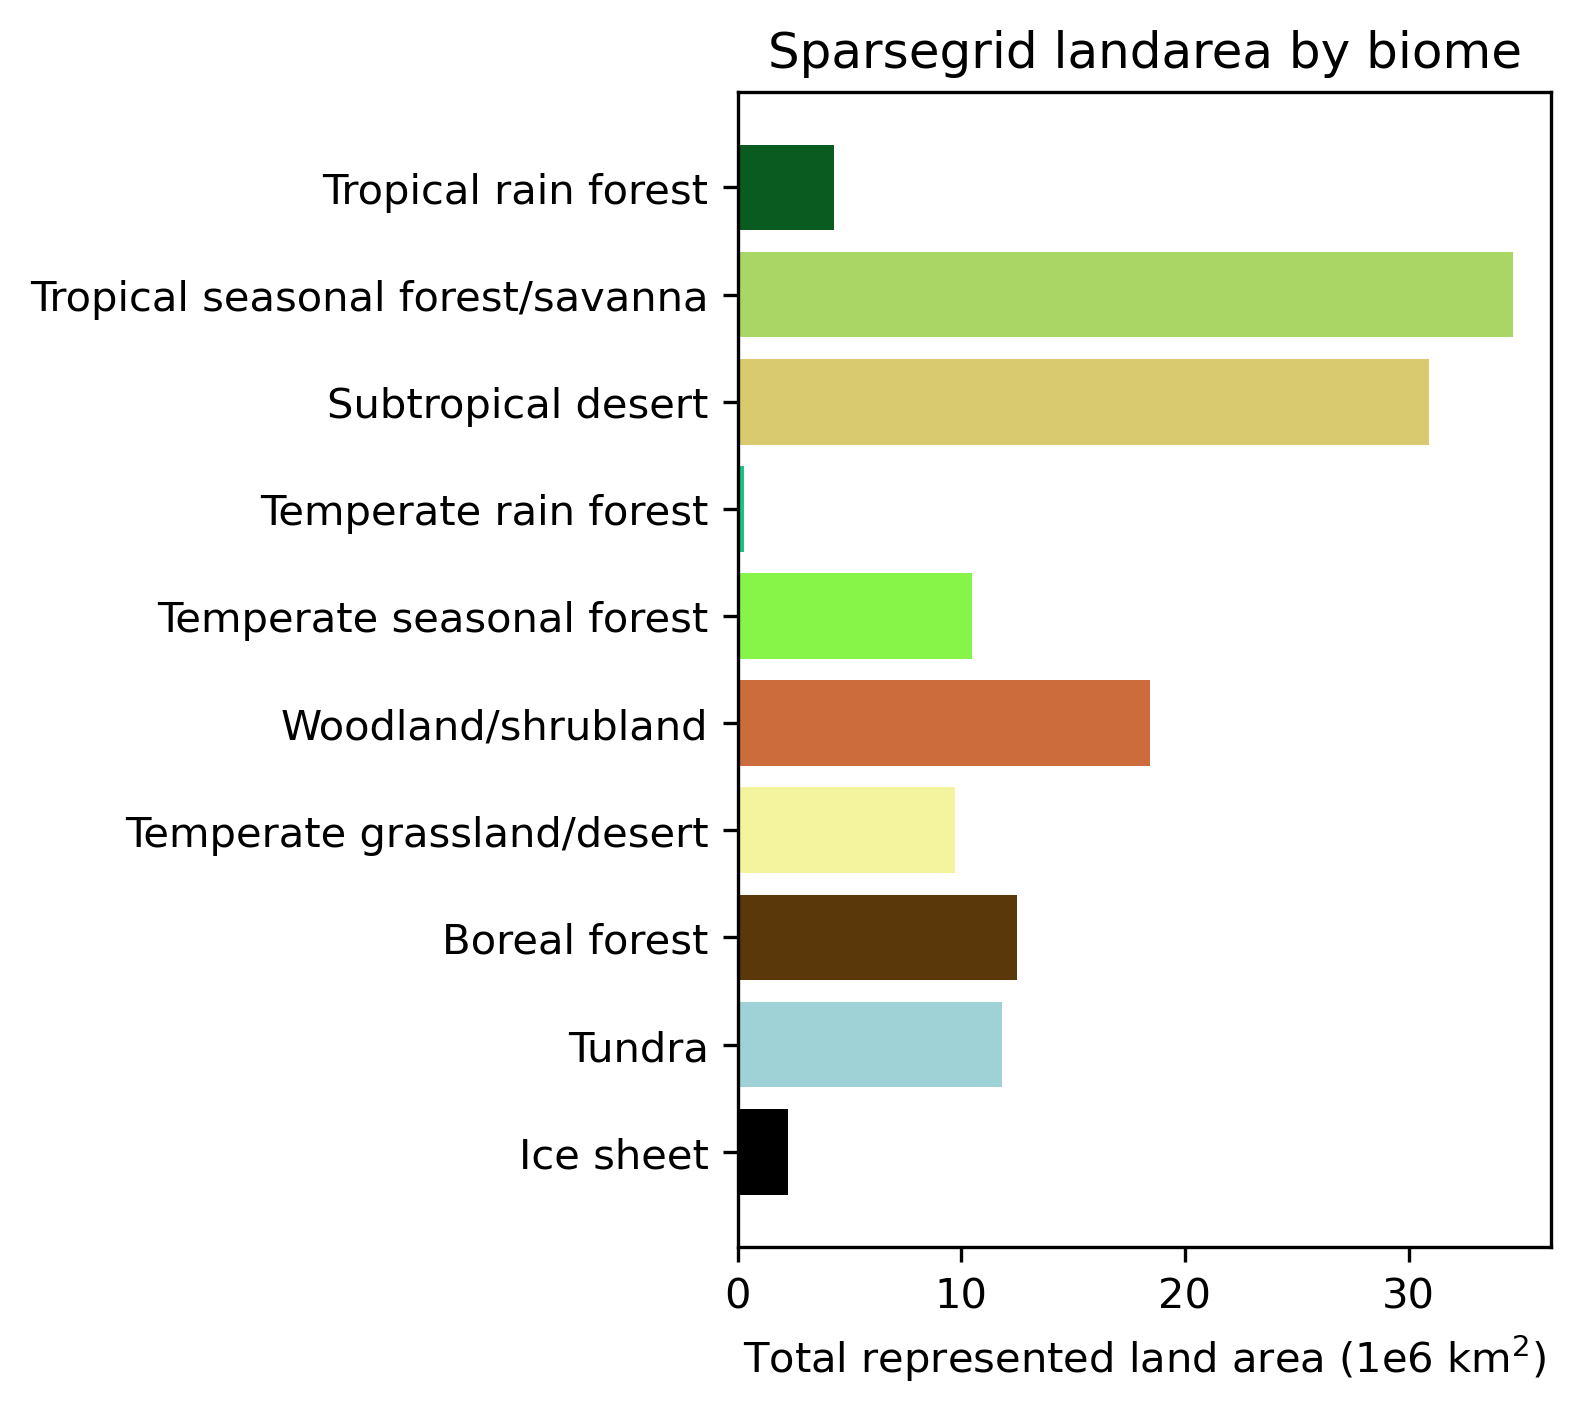
\includegraphics[width=23pc]{../figs/supp/biome_areas.png}
\caption{Total represented land area associated with each of the ten Whittaker biomes utilizing the CLM5.1 sparsegrid.}
\label{supp:whit3}
\end{figure}




\begin{figure}[h]
\centering
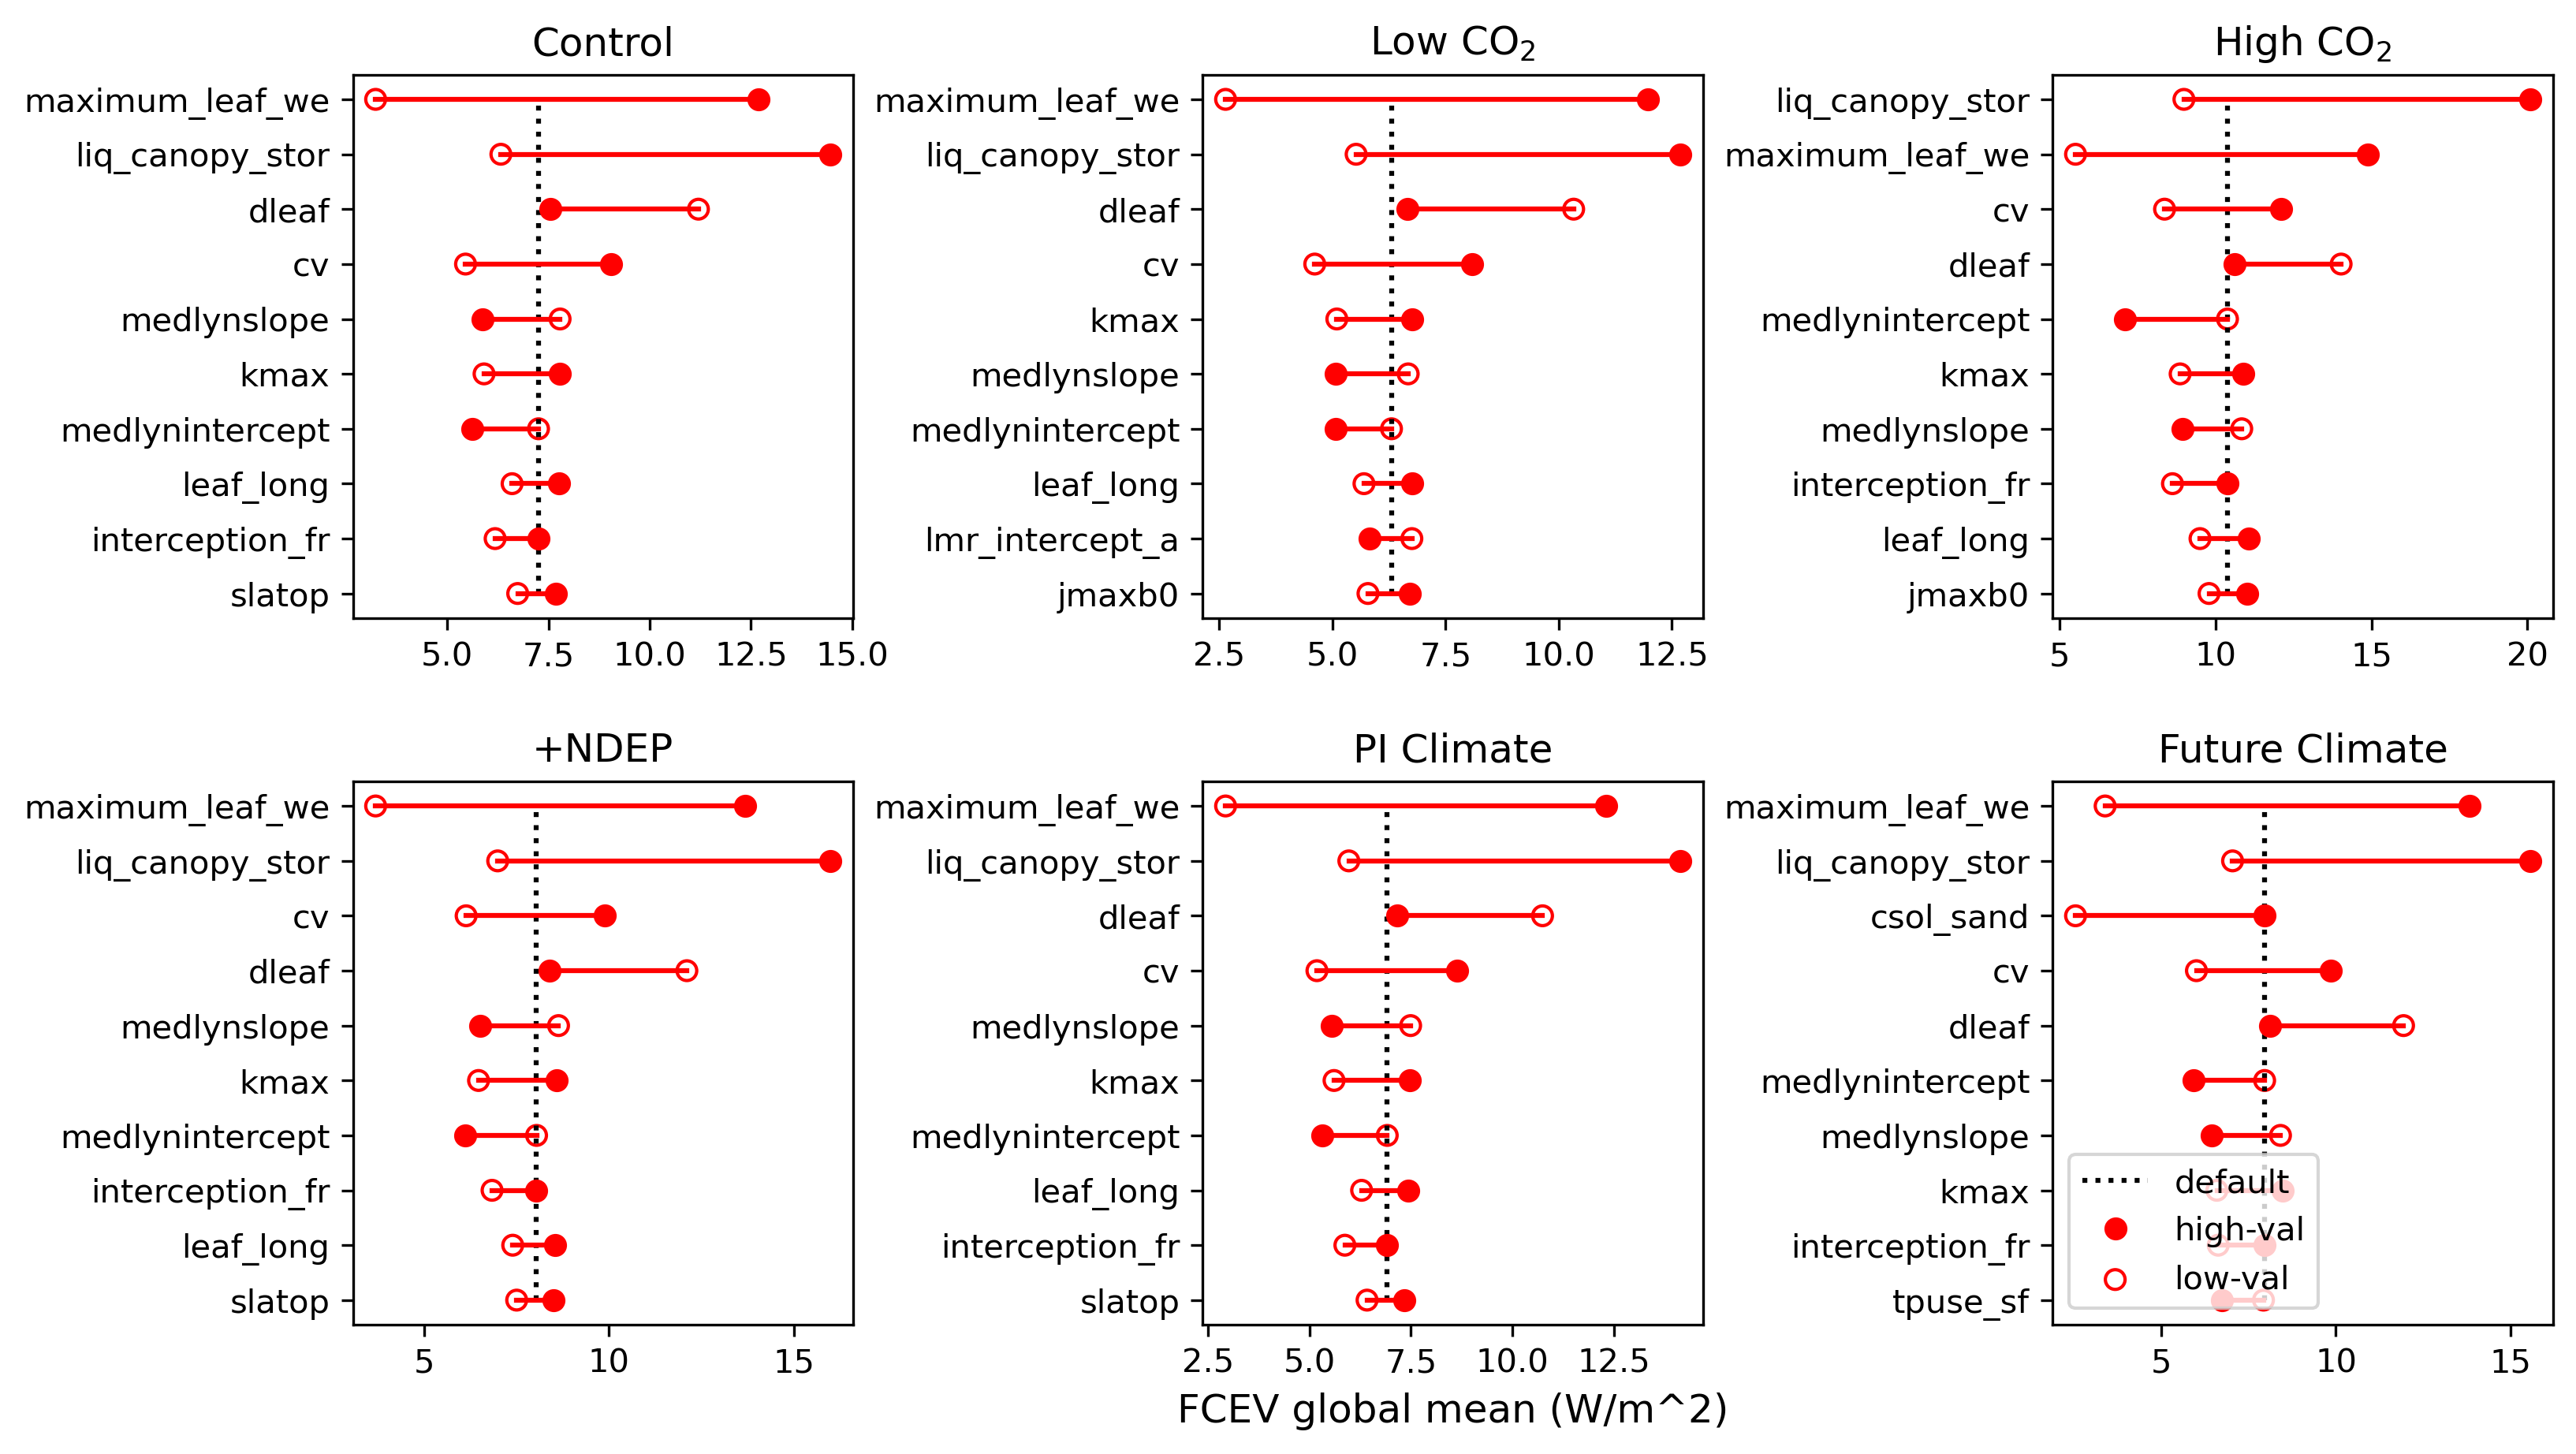
\includegraphics[width=\textwidth]{../figs/supp/FCEV_global_mean.png}
\caption{Global mean canopy evaporation (FCEV) parameter rankings across the six forcing scenarios.}
\label{supp:fcev}
\end{figure}






\end{document}
